\chapter{Evaluation}

First of all, the accuracy of the model was tested agaist the testing subset provided by the used dataset. The following groups of images show the loss (left) and
the accuracy (right) at each epoch.

\begin{figure}[H]
\centering
\begin{minipage}{.45\textwidth}
  \centering
  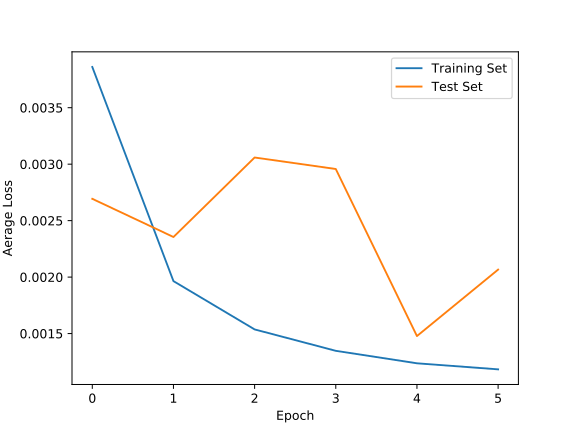
\includegraphics[width=\linewidth]{model_losses_default.png}
  \caption{Default Model Losses - Training}
\end{minipage}
\begin{minipage}{.45\textwidth}
  \centering
  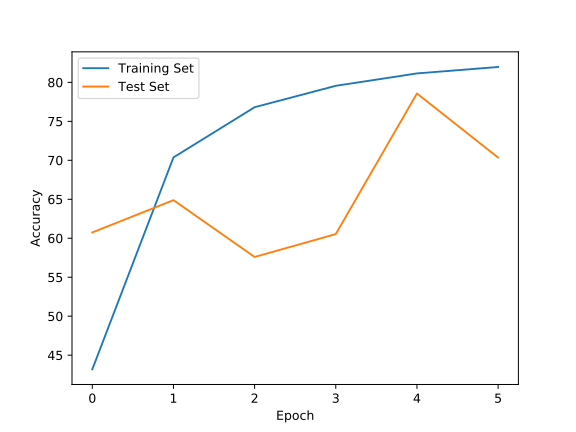
\includegraphics[width=\linewidth]{model_accuracies_default.png}
  \caption{Default Model Accuracies - Training}
\end{minipage}
\end{figure}

Interestingly, the testing accuracy seems to fluctuate and even decreases by a bit at the end while the training accuracy still keeps growing. But still, with
the testing dataset reaching a 78.1\% accuracy and the training dataset reaching a accuracy of 82.5\%, the goal is definetly reached. For reference, the same model
is tested against the validation dataset to see if there are differences in data quality.

\begin{figure}[H]
\centering
\begin{minipage}{.45\textwidth}
  \centering
  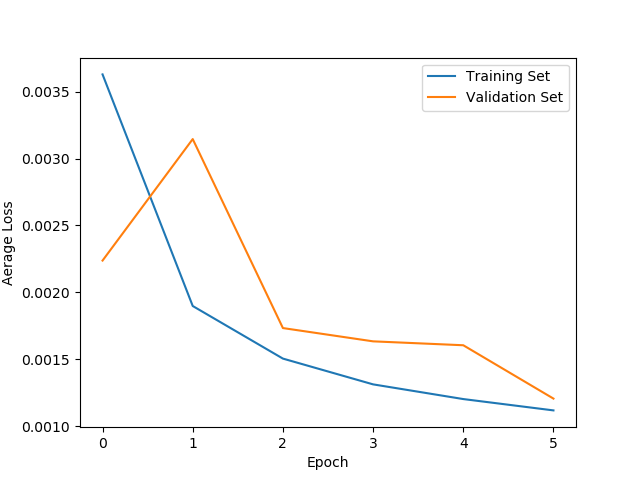
\includegraphics[width=\linewidth]{model_losses_validation.png}
  \caption{Default Model Losses - Validation}
\end{minipage}
\begin{minipage}{.45\textwidth}
  \centering
  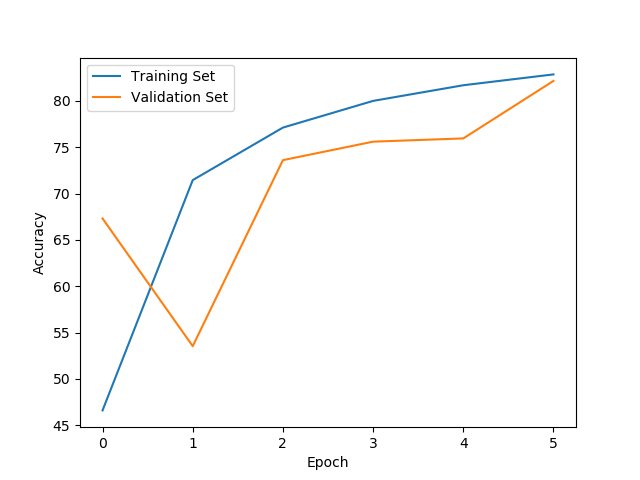
\includegraphics[width=\linewidth]{model_accuracies_validation.png}
  \caption{Default Model Accuracies - Validation}
\end{minipage}
\end{figure}

Here, a bit smoother curve for the validation dataset can be seens with the training set reaching 82.9\% and the validation set reaching 82.2\%. With the relativly small epoch
count and it being relativly close to the testing accuracy, it is concluded that no difference in data quality exists. In the next step, the the model is evaluated
with background noise. The following table shows the maximum accuracies for different noises provided by the dataset mixed into the original testing audio at different percentages.

\begin{table}[H]
  \begin{center}
    \begin{tabular}{l|l|l|l}
      Percentage & Exercise Bike & Running Tap & White Noise\\\hline
      50 & 76.9 & 68.8 & 70.1\\
      75 & 66.1 & 62.8 & 55.9\\
    \end{tabular}
    \caption{Background Noise Accuracies}
  \end{center}
\end{table}

The accuracies seem still unreasonably high, even when the background noise is mixed in with a majority. This might be because of all the noises being
relativly constant with no sudden spikes. Also, there is no guarantee that amplitudes (or audio volume) for the original audio and the background noise are equal. So 
even when mixed at a equal rate, they might still not have a equal influence on the overall signal. And as constant noise doen´t alter the waveform very much, the 
model can still recognize its shape.

The last evaluation will focus on data from a more realistic environment. The model will be tested with a real microphone and each label listed below will be repeated
10 times and the accuracies will be averaged. If a command is incorrectly predicted, its accuracy is counted as 0\%.

\begin{table}[H]
  \begin{center}
    \begin{tabular}{l|l|l|l|l}
    Criterium & Six & On & Zero & Yes\\\hline
    Average & 38.6 & 18.9 & 18.8 & 24.3\\
    Highest & 62 & 48 & 26 & 82\\
    Correct & 9 & 6 & 10 & 8\\
    Most Similiar & Sheila & One & - & Six\\
    \end{tabular}
    \caption{Realistic Environment Accuracies}
  \end{center}
\end{table}

It is shown, that commands are correctly predicted, but the accuracies are way lower than the ones found with the provided dataset. Especially commands that have a simmilar
command ("On" vs "One") have very low accuracies. Also noted should be the very high fluctuation between iterations of the same word. All words were repeated in the same tone and speed, the waveforms
should be almost equal (to a human at least). But still, the command "Yes" for eample achieved a 82\% accuracy during one run and a 0\% accuracy during another.
